\documentclass[11pt]{article}
\usepackage[margin=1in]{geometry}
\usepackage{amsmath,amssymb}
\usepackage{graphicx}
\usepackage{booktabs}
\usepackage[colorlinks=true,linkcolor=blue,citecolor=blue,urlcolor=blue]{hyperref}

% --- the only two lines to edit before submission ---
\newcommand{\authorname}{Singularity}
\newcommand{\affiliation}{}

\title{A compact learned Fourier correction\\ for two-dimensional smoke simulation}
\author{\authorname\\ \small \affiliation}
\date{\today}

\begin{document}
\maketitle

\begin{abstract}
A neural operator placed after a complete smoke solver can cost more than simply using a finer classical grid. We
instead fold a learned Fourier correction with eight coefficients into the diffusion transform of a one-step
transport solver with a midpoint trajectory. On 64 held-out synthetic smoke scenes the method ran at 0.889~ms per
frame on one CPU and reduced mean density error by 8.8\% relative to the best classical configuration within the same
latency band (0.955~ms), with a paired interval of 4.6 to 13.1\%; it improved 49 of 64 scenes and ran 55 times faster
than the fine reference. The criterion was fixed before the test. The gain grows with the accuracy of the reference
(9.8\% against a $256\times256$ reference on eight predetermined scenes, 3.0\% against a coarser $144\times144$ one),
consistent with the correction recovering detail that coarse grids lose. The learned part adds only eight numbers to
an existing solver.
\end{abstract}

\section{Introduction}
Semi-Lagrangian transport makes smoke simulation cheap enough for computer graphics~\cite{stam}; a bounded MacCormack
scheme improves accuracy at the cost of extra interpolation and limiting~\cite{selle}. Fourier neural
operators~\cite{li} learn field-to-field maps in frequency space and are a natural candidate for correcting a coarse
solver. The practical question is not whether such a correction lowers error, but whether it does so at a cost
below that of a finer classical grid. We study a design in which the learned correction reuses the Fourier
transforms the solver already computes for diffusion, so it adds almost no time.

\section{Methods}
\paragraph{Smoke model.} Buoyant smoke in a two-dimensional periodic square without obstacles. The state is density
and vorticity; a divergence-free velocity is recovered through a Fourier stream-function solve, with a uniform lateral
wind. A moving Gaussian source injects density and the horizontal density gradient drives vorticity. Viscosity and
diffusion are Fourier multipliers. Scene seeds vary wind, source and initial vortices; one frame lasts 0.045 time
units, and all outputs are compared on a $144\times144$ grid.

\paragraph{Transport and learned correction.} The velocity at the middle of each interval is extrapolated as
$\tilde u_j=1.5u_j-0.5u_{j-1}$ and the solver backtraces from $x$ to $x-\Delta t\,\tilde u_j(x-\frac12\Delta
t\,\tilde u_j(x))$. After interpolation, source and forces, the same Fourier transforms used for diffusion apply the
correction. For channel $c$ and axis $a$, with $s_a=\sin^2(\pi k_a/n)$ and $q_a$ the spatial mean of
$4f_a(1-f_a)$, where $f_a$ is the fractional departure displacement in cells,
\begin{equation}
 M_c(k)=1+\mathrm{clip}[\frac{1}{2}\sum_{a\in\{x,y\}}q_a\,(w_{c,a,1}s_a+w_{c,a,2}s_a^2),\ -0.18,\ 0.55].
\end{equation}
The eight weights are fitted by regularised least squares against the next reference state on 48 training scenes.
The filter is stored as two axis profiles; on development states it differs from the unfactored form by at most
$3.8\times10^{-6}$.

\paragraph{Comparators and timing.} Bounded MacCormack and linear or cubic interpolation with Euler, midpoint and
temporal backtracing, over grid sizes from 48 to 144. The matched-cost comparator is the lowest-error classical method
whose median step time is within 115\% of the learned method. Warm timings on an AMD Ryzen~5 5625U include simulation
and resampling to the common grid; method order is randomised per scene.

\paragraph{Study sequence.} A first pilot (a two-layer Fourier network correcting a finished MacCormack step) and a
second design (a spectral corrector on a single interpolated transport) were each tested on 24 new scenes and failed
their criteria. The present design, with the $96\times96$ grid and filter strength chosen on 12 development scenes,
then failed a first test of 64 scenes against a $144\times144$, four-substep reference, while an eight-scene check
with a finer $192\times192$ reference favoured it. A new test was therefore fixed in writing before running: frozen
model, 64 new scenes (32 with winds inside the training range, 32 above), primary reference $192\times192$ with eight
substeps, the $144\times144$ reference reported in parallel, and a $256\times256$, 16-substep check on eight scenes
chosen in advance. Primary criterion: at least 5\% lower mean per-scene density RMSE than the matched-cost comparator,
a positive lower bound of a paired stratified bootstrap interval, and at least a twofold speed-up over the fine
reference. Secondary: at least 10\% lower median time than the classical $112\times112$ temporal solver, with the
interval on the relative error change below $+5\%$.

\section{Results}
\begin{table}[h]
\centering
\begin{tabular}{lrrrr}
\toprule
method & grid & median ms & RMSE (ref.\ 192) & RMSE (ref.\ 144) \\
\midrule
temporal linear, no filter & $96^2$ & 0.802 & 0.03115 & 0.02999 \\
temporal linear (matched cost) & $108^2$ & 0.955 & 0.02779 & 0.02674 \\
temporal linear & $112^2$ & 1.031 & 0.02690 & 0.02590 \\
learned Fourier correction & $96^2$ & \textbf{0.889} & \textbf{0.02535} & 0.02594 \\
\bottomrule
\end{tabular}
\caption{Held-out rollouts on 64 scenes of 40 frames; RMSE averaged per scene. The $108\times108$ row is the strongest
classical method in the primary latency band.}
\label{tab:results}
\end{table}

\begin{table}[h]
\centering
\begin{tabular}{lrrr}
\toprule
reference & error reduction vs matched cost & paired 95\% interval & scenes improved \\
\midrule
$192\times192$, 8 substeps (primary) & \textbf{8.8\%} & 4.6 to 13.1\% & 49 / 64 \\
$144\times144$, 4 substeps & 3.0\% & $-1.2$ to 7.3\% & 39 / 64 \\
$256\times256$, 16 substeps (8 scenes) & 9.8\% & -- & -- \\
\bottomrule
\end{tabular}
\caption{Dependence on the numerical reference. On the eight-scene check the mean errors are 0.03061 (learned) and
0.03394 (matched cost).}
\label{tab:reference}
\end{table}

\begin{figure}[h]
\centering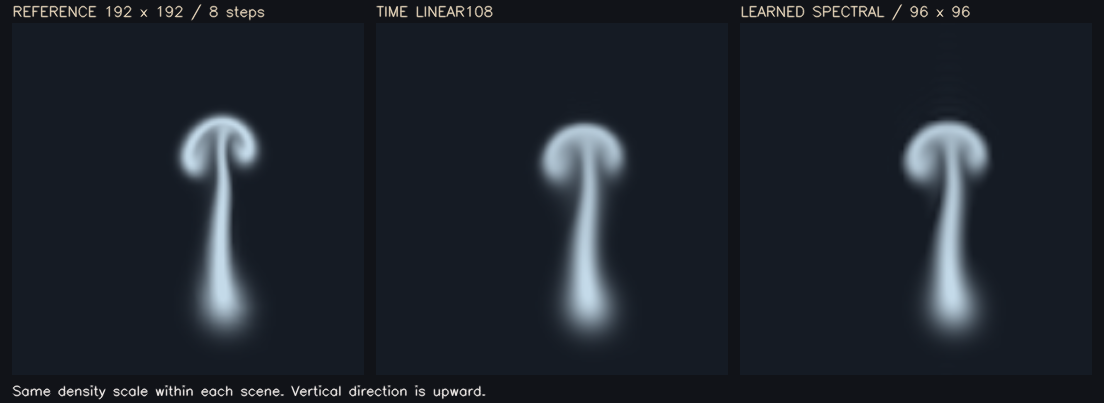
\includegraphics[width=.93\linewidth]{fig_frame.png}
\caption{One frame of the first held-out scene on a common density scale. Left: fine reference. Middle: strongest
classical solver at comparable latency. Right: learned correction.}
\label{fig:frame}
\end{figure}

\begin{itemize}
\item \textbf{Primary criterion met.} 8.8\% lower error than the best classical solver at comparable cost, with a
55-fold speed-up over the fine reference (Table~\ref{tab:results}).
\item \textbf{The filter matters.} On the same $96\times96$ grid and trajectory, the learned method has 18.6\% lower
error than the solver with its filter disabled, so the gain is not only the better trajectory.
\item \textbf{Secondary criterion met.} Against the classical $112\times112$ solver the method saves 13.8\% of median
time while its error is 5.8\% lower (upper interval endpoint $-1.6\%$).
\item \textbf{Larger against finer references.} 9.8\% against the $256\times256$ check, 3.0\% against the coarser
$144\times144$ reference, where the interval includes zero (Table~\ref{tab:reference}).
\end{itemize}

\section{Discussion}
The advance comes from combining a better departure trajectory with a learned correction that reuses an existing
transform, so the correction is almost free in time. The finer the reference, the clearer the advantage, which is
consistent with the correction recovering detail that a coarse reference itself lacks. Because the filter lives
inside transforms that diffusion already needs, the same idea can be tried in any spectral smoke solver, with
three-dimensional scenes and obstacles as the next steps.

\paragraph{Limitations.} Synthetic periodic smoke without obstacles, one CPU and 40-frame sequences. The finer primary
reference was adopted after a first test against the coarser one failed; the confirming test used new scenes and a
frozen model.

\paragraph{Reproducibility.} \texttt{experiment.py} runs, in order, development, the first test, the test with the
finer reference and the figure; the two earlier designs are kept in \texttt{code/} (top level and
\texttt{retry/}) with their own scripts. \texttt{results.json} contains all five stages: the two earlier designs,
the first test, the confirmation and the $256\times256$ check. Scene seeds, weights, per-scene errors and frame
timings are included.

\paragraph{Origin of the question.} The question came from an automated forecast (Singularity v1, registered on 30
October 2026 with a SHA-256 fingerprint) that neural operators would enter computer graphics. The forecast concerned
the arrival of the method, not the result of this study.

\begin{thebibliography}{9}
\bibitem{stam} J.~Stam, Stable fluids, \emph{Proc.\ SIGGRAPH} (1999), doi:10.1145/311535.311548.
\bibitem{selle} A.~Selle, R.~Fedkiw, B.~Kim, Y.~Liu and J.~Rossignac, An unconditionally stable MacCormack method,
\emph{Journal of Scientific Computing} 35, 350--371 (2008), doi:10.1007/s10915-007-9166-4.
\bibitem{li} Z.~Li et al., Fourier neural operator for parametric partial differential equations, \emph{ICLR} (2021),
arXiv:2010.08895.
\end{thebibliography}
\end{document}
